\section{Usuario Registrado}

\subsection{P\'{a}gina Principal}
El usuario que haya iniciado sesi\'{o}n ser\'{a} redireccionado autom\'{a}ticamente a la p\'{a}gina principal de la web, en la cual podr\'{a} observar que pr\'{a}cticamente no ha cambiado, excepto por su barra de navegaci\'{o}n, que le acompa\~{n}ar\'{a} en todo el sitio web. \\

Aparece una nueva opci\'{o}n de navegaci\'{o}n, la cual permite visitar el perfil de usuario y consultar sus peticiones sobre anuncios publicados. Tambi\'{e}n se ha sustitu\'{i}do el inicio de sesi\'{o}n por el cierre de sesi\'{o}n, para poder salir del sistema.

\begin{figure}[h!]
\centering
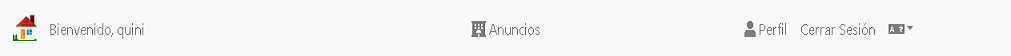
\includegraphics[width=1\textwidth]{Img/ManualUsuario/USER_MENU.png}
\end{figure}

Puede observarse que, en la parte izquierda, el usuario recibe un mensaje de bienvenida personalidado.

\begin{figure}[h!]
\centering
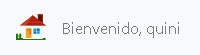
\includegraphics[width=.5\textwidth]{Img/ManualUsuario/USER_MENU_SALUDO.png}
\end{figure}

En lo referente a las b\'{u}squedas y listados de anuncios, las vistas no cambian con respecto al usuario no registrado, de manera que se proceder\'{a} a comentar las diferencias con respecto al anterior.

\subsection{Anuncios}
En las consultas propias de los anuncios se pueden apreciar una serie de caracter\'{i}sticas diferentes a las ofrecidas para un usuario no logueado en el sistema, o GUEST.\\

Aparte de que los datos del anuncio se muestren de la misma manera, las opciones del men\'{u} lateral ofrecen ahora la posibilidad de denunciar el anuncico, contactar con el anunciante realizando una petici\'{o}n, as\'{i} como valorar positiva o negativamente el  mismo. En este caso, el usuario registrado podr\'{a} consultar el perfil de usuario del anunciante haciendo click en su nombre.

\begin{figure}[h!]
\centering
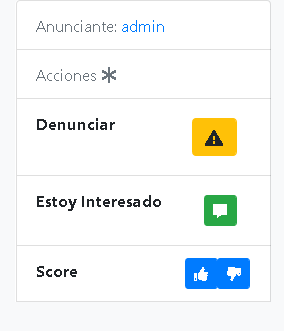
\includegraphics[width=.3\textwidth]{Img/ManualUsuario/LATERAL_AD_USER_NO_PETICION.png}
\end{figure}

Una vez se haya realizado una petici\'{o}n sobre un anuncio, esta opci\'{o}n se ver\'{a} sustitu\'{i}da por el siguiente mensaje:
\begin{figure}[h!]
\centering
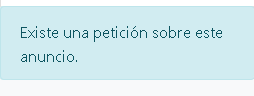
\includegraphics[width=.3\textwidth]{Img/ManualUsuario/LATERAL_AD_USER_PETICION.png}
\end{figure}

En la secci\'{o}n de mensajes, ahora se permite que se env\'{i}e un comentario sobre el anuncio. Este comentario ser\'{a} p\'{u}blico, por tanto, se podr\'{a} denunciar por otros usuarios del mismo modo que el usuario en cuesti\'{o}n pueda realizar una petici\'{o}n de denuncia sobre aquel comentario que desee.


\begin{figure}[h!]
\centering
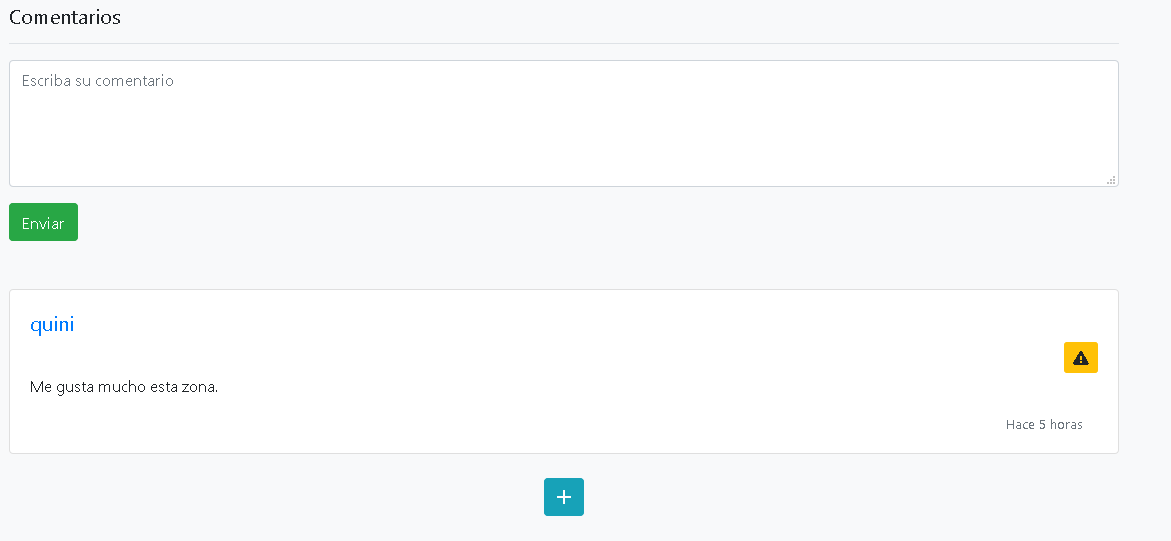
\includegraphics[width=1\textwidth]{Img/ManualUsuario/USER_AD_COMMENTS.png}
\end{figure}

\subsection{Perfil de Usuario}

Al acceder desde la opci\'{o}n del men\'{u} principal con el nombre 'Perfil' el usuario dispondr\'{a} de un peque\~{n}o formulario con sus datos editables y una peque\~{n}a columna que muestre las actividades, como la cantidad de anuncios publicados y comentarios. \\

A diferencia de los comentarios, los anuncios podr\'{a}n  ser consultados, list\'{a}ndose del mismo modo que en la p\'{a}gina de listado, en caso de existir m\'{a}s de uno, haciendo click sobre la opci\'{o}n pertinente. 


\begin{figure}[h!]
\centering
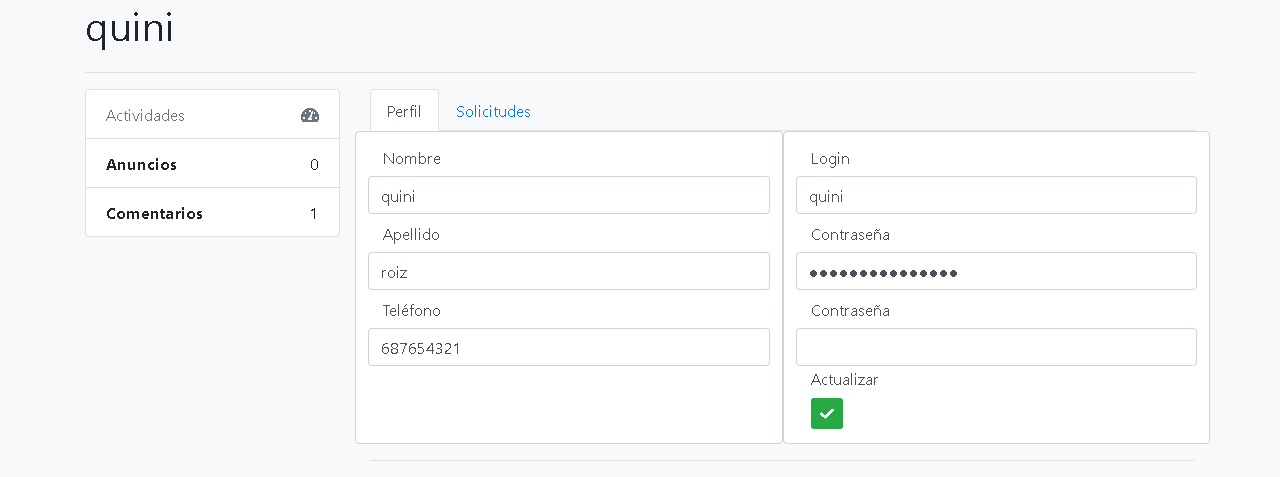
\includegraphics[width=.9\textwidth]{Img/ManualUsuario/USER_PROFILE_EDIT.png}
\end{figure}

Justo encima de la tarjeta de perfil, se encuentra la pesta\~{n}a de solicitudes, donde, al hacer click,  el usuario dispondr\'{a} de una tabla  podr\'{a} listar y gestionar sus solicitudes existentes sobre alg\'{u}n anuncio que hubiera publicado. En esta tabla se muestra el anuncio asociado a cada petici\'{o}n y el usuario que la cre\'{o}, adem\'{a}s del tiempo pasado desde entonces. Se ofrece tambi\'{e}n un bot\'{o}n para visualizar el contenido de la petici\'{o}n.

\begin{figure}[h!]
\centering
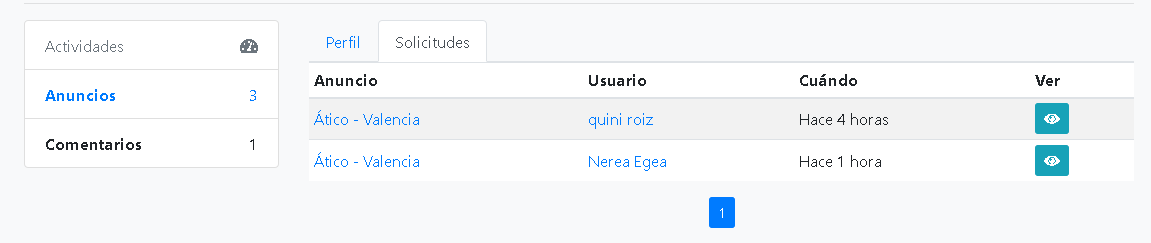
\includegraphics[width=1\textwidth]{Img/ManualUsuario/USER_REQUESTS.png}
\end{figure}

Haciendo click en el nombre del anuncio se redirigir\'{a} al anuncio en cuesti\'{o}n para poder observarlo. Del mismo modo, al hacer click en un usuario, se podr\'{a} ver el perfil del mismo. \\


Si se accede al bot\'{o}n 'Ver' de una fila de peticiones, se abrir\'{a} un modal con el contenido de la petici\'{o}n, en donde se encuentran el accedo al perfil del usuario que realiz\'{o} la petici\'{o}n, los datos de contacto (al hacer click sobre el correo se abrir\'{a} la aplicaci\'{o}n que se tenga por defecto en el sistema para enviarle un correo electr\'{o}nico personal) y el contenido de la propia petici\'{o}n a modo de texto. \\

En la zona derecha, se puede observar un bot\'{o}n amarillo que permite denunciar la petici\'{o}n, en caso de que sea inadecuada. Debajo de este, se ofrecen las posibilidades de aceptar y rechazar petici\'{o}n, con sus respectivos botones (en rojo rechazar y en verde aceptar). Debajo de estos botones la fecha de registro de la petici\'{o}n.

\begin{figure}[h!]
\centering
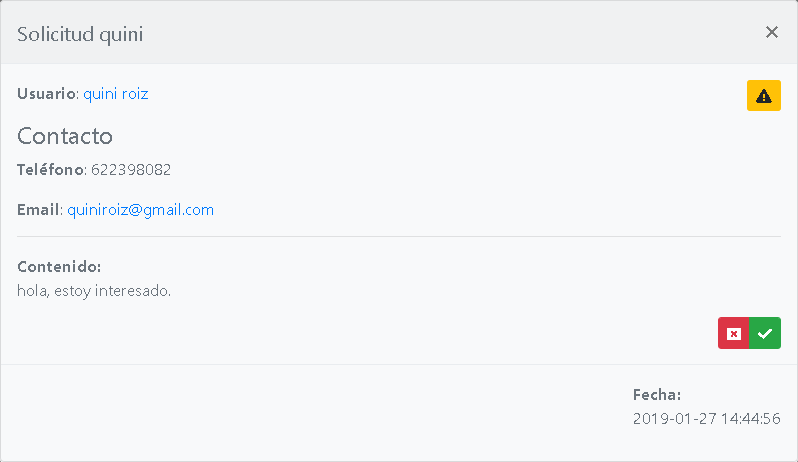
\includegraphics[width=.6\textwidth]{Img/ManualUsuario/USER_REQUEST_READ.png}
\end{figure}

\subsubsection{Perfil de otros usuarios}
Si es el perfil de otro usuario el que se consulta, el aspecto ser\'{a} muy similar al visto en el anterior punto, salvo que no se listan las peticiones (es algo privado) y los datos son s\'{o}lamente de lectura. 

Encima del nombre, a la derecha, aparecer\'{a} un bot\'{o}n que permite denunciar al usuario en caso de mal comportamiento. \\

\begin{figure}[h!]
\centering
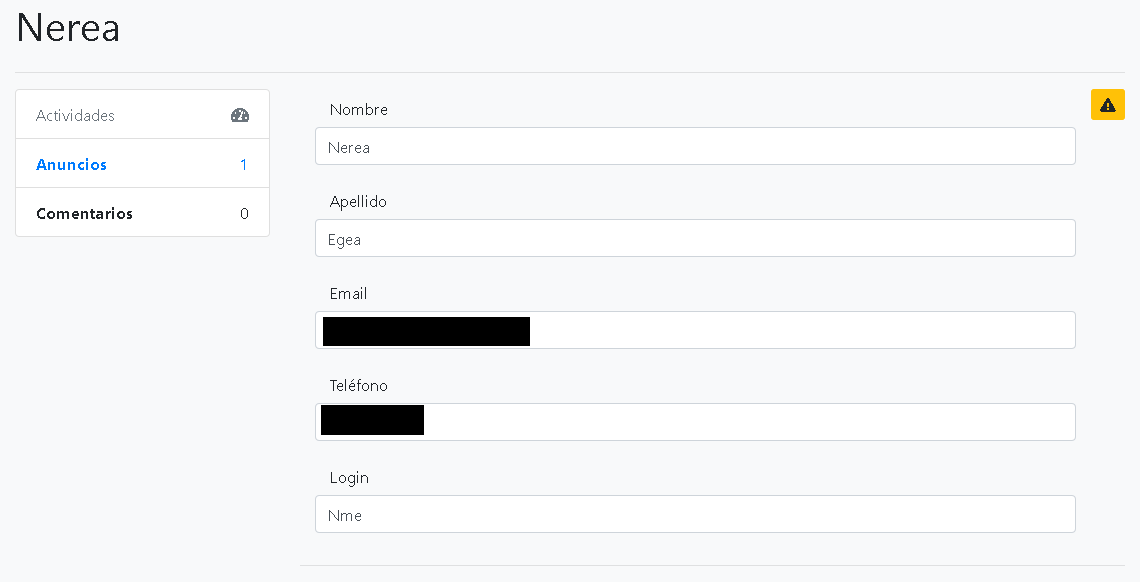
\includegraphics[width=.8\textwidth, height=.2\textheight]{Img/ManualUsuario/PERFIL_OTHER.png}
\end{figure}

\subsection{Crear una denuncia}
Sea el caso de denunciar un comentario, un anuncio, un usuario o una petici\'{o}n, el formulario de denuncia es el mismo, solicitando el t\'{i}tulo y una detallada descripci\'{o}n del motivo de denuncia. 

\begin{figure}[h!]
\centering
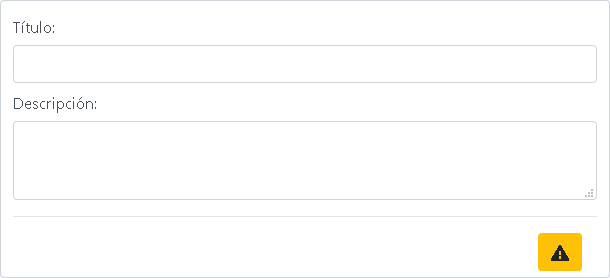
\includegraphics[width=.5\textwidth]{Img/ManualUsuario/DENUNCIA.png}
\end{figure}




